%\documentclass[12pt, preprint,numberedappendix]{emulateapj}
%\documentclass[12pt, preprint]{aastex}
%\documentclass[dvips,12pt]{article}
\documentclass[apj]{emulateapj}

\newcommand\submitms{n}		% set to y to follow AAS ``ms'' names, etc.
\newcommand\bibinc{n}		% set to y if bib pasted in .tex, set to n to use bibtex


%\usepackage{pdfsync}
\usepackage{subeqnarray}
\usepackage{natbib}
\usepackage{color}
\usepackage[utf8]{inputenc}

\bibliographystyle{apj}

\newcommand{\ie}{i.e.\ }
\newcommand{\eg}{e.g.\ }
\newcommand{\p}{\partial}
\newcommand{\brak}[1]{\langle #1\rangle}


\newcommand{\gcc}{\;\mathrm{g\; cm^{-3}}}
\newcommand{\gsc}{\;\mathrm{g\; cm^{-2}}}
\newcommand{\cm}{\; {\rm cm}}
\newcommand{\mm}{\; {\rm mm}}
%\newcommand{\ps}{\; {\rm s^{-1}}}
\newcommand{\km}{\; {\rm km}}
\newcommand{\au}{\; \varpi_{\rm AU}}
\newcommand{\AU}{\; {\rm AU}}
\def\K{\; {\rm K}}

\newcommand{\vcs}[1]{\mbox{\boldmath{$\scriptstyle{#1}$}}}
\newcommand{\vc}[1]{\mbox{\boldmath{$#1$}}}
\newcommand{\nab}{\vc{\nabla}}
\DeclareMathSymbol{\varOmega}{\mathord}{letters}{"0A}
\DeclareMathSymbol{\varSigma}{\mathord}{letters}{"06}
\DeclareMathSymbol{\varPsi}{\mathord}{letters}{"09}

\newcommand{\Eq}[1]{Equation\,(\ref{#1})}
\newcommand{\Eqs}[2]{Equations (\ref{#1}) and~(\ref{#2})}
\newcommand{\Eqss}[2]{Equations (\ref{#1})--(\ref{#2})}
\newcommand{\App}[1]{Appendix~\ref{#1}}
\newcommand{\Sec}[1]{Sect.~\ref{#1}}
\newcommand{\Chap}[1]{Chapter~\ref{#1}}
\newcommand{\Fig}[1]{Fig.~\ref{#1}}
\newcommand{\Figs}[2]{Figs.~\ref{#1} and \ref{#2}}
\newcommand{\Figss}[2]{Figs.~\ref{#1}--\ref{#2}} 
\newcommand{\Tab}[1]{Table \ref{#1}}

\definecolor{gray}{gray}{0.5}
\newcommand{\emgr}[1]{\emph{ \color{gray} #1}}


%\newenvironment{packed_item}{
%\begin{itemize}
%  \setlength{\itemsep}{1pt}
%  \setlength{\parskip}{0pt}
%  \setlength{\parsep}{0pt}
%}{\end{itemize}}

\begin{document}

%\slugcomment{Draft Modified \today}


\title{The Role of Ice Compositions and Morphology for Snowlines and the C/N/O Ratios in Active Disks}

\author{Ana-Maria A. Piso\altaffilmark{1}, Karin I. \"Oberg\altaffilmark{1}, \& Jamila Pegues\altaffilmark{2}}
\altaffiltext{1}{Harvard-Smithsonian Center for Astrophysics, 60 Garden Street, Cambridge, MA 02138}
\altaffiltext{2}{Department of Astrophysical Sciences, Princeton University}


\begin{abstract}
...
\end{abstract}

\section{Introduction}

\emgr{Background info. Importance of volatiles in disks and planetary atmospheres, detections of snowlines in disks, C/O ratios etc. State again the importance of radial drift and gas accretion on the snowline locations, and that a systematic study of the combination of these two particular effects across the disk has not been done before. Then transition to the fact that we provide such a systematic study in Paper I and in this paper. Here, we expand the model of Paper I by making three additions: (1) we add N and CH4 in the static chemistry model, and explore how different abundances of CH4 and of the N main carriers (N2 and NH3) affect the C/O  and N/O ratios, (2) we quantify the effect of radial drift and gas accretion on the N2, CH4 and NH3 snowline locations, and (3) we explore how different binding energies of CO and N2 affect their snowline locations.}

\section{Model Review}

\emgr{Review disk models, desorption model, relevant timescales. State that we use a steady-state disk for the coupled drift-desorption evolution, since it is the most realistic, therefore only summarize the static and steady-state (viscous) disk. Summarize the findings of Paper I, i.e. particles of certain sizes desorb instantaneously and at a fixed particle size dependent location.}

\section{CH4 and C/O Ratios}

\emgr{Discuss observed abundances for CH4 and the choices that we make (no CH4, median value, maximum value). State that desorption energies for H2O, CO2 and CH4 are well constrained experimentally, and that the CO2 and CH4 binding energies are only weakly dependent on whether it's pure CO2/CH4 or combined with H2O, but that is not the case for CO (and N2 as we will show in the next section). Present new binding energies for CO as pure ice and mixed with water. Show Figure 1 and discuss how different CH4 abundances and binding energies affect snowline locations and C/O ratio: CO-H2O mixture (though I think it's rather CO layered on top of H2O) moves the CO snowline inward by $\sim$40 AU (will calculate percentages too); the maximum reasonable abundance of CH4 changes the C/O ratio by less than 10\%. Show Figure 2 and quantify the effect of drift and accretion on the CH4 snowline compared to a static disk. While CH4 has only a modest effect on the C/O ratio in a static disk, this effect may be larger in a viscous disk, as the C gas abundances inside the CH4 snowline may be enhanced due to the differential motion of the desorbed ices and overall nebular gas (refer to Paper I). In this study, however, we neglect these effects and therefore do not include CH4 in estimating the C/O ratio (as an aside, the figures that include CH4 in the C/O ratio with drift and desorption are quite messy due to snowlines overlapping). Show Figure 3 and estimate the difference between CO-H2O and CO pure ice snowlines in the case of drift and accretion, as well as the comparisons for the static disk for the CO snowline.}

\begin{figure}[h!]
\centering
\includegraphics[width=0.5\textwidth]{../../figs/C_O_ratio_CH4_test.pdf}
%\vspace{-0.5in}
\caption{C/O ratio in a static disk for different CH4 abundances and CO binding energies...} 
\label{fig:COstatic}
\end{figure}

\begin{figure}[h!]
\centering
\includegraphics[width=0.5\textwidth]{../../figs/desorption_distance_CH4_steady.pdf}
%\vspace{-0.5in}
\caption{Desorption distance as a function of initial distance for CH4.... Drift and gas accretion move the CH4 snowline inward by x\%.} 
\label{fig:CH4}
\end{figure}

\begin{figure}[h!]
\centering
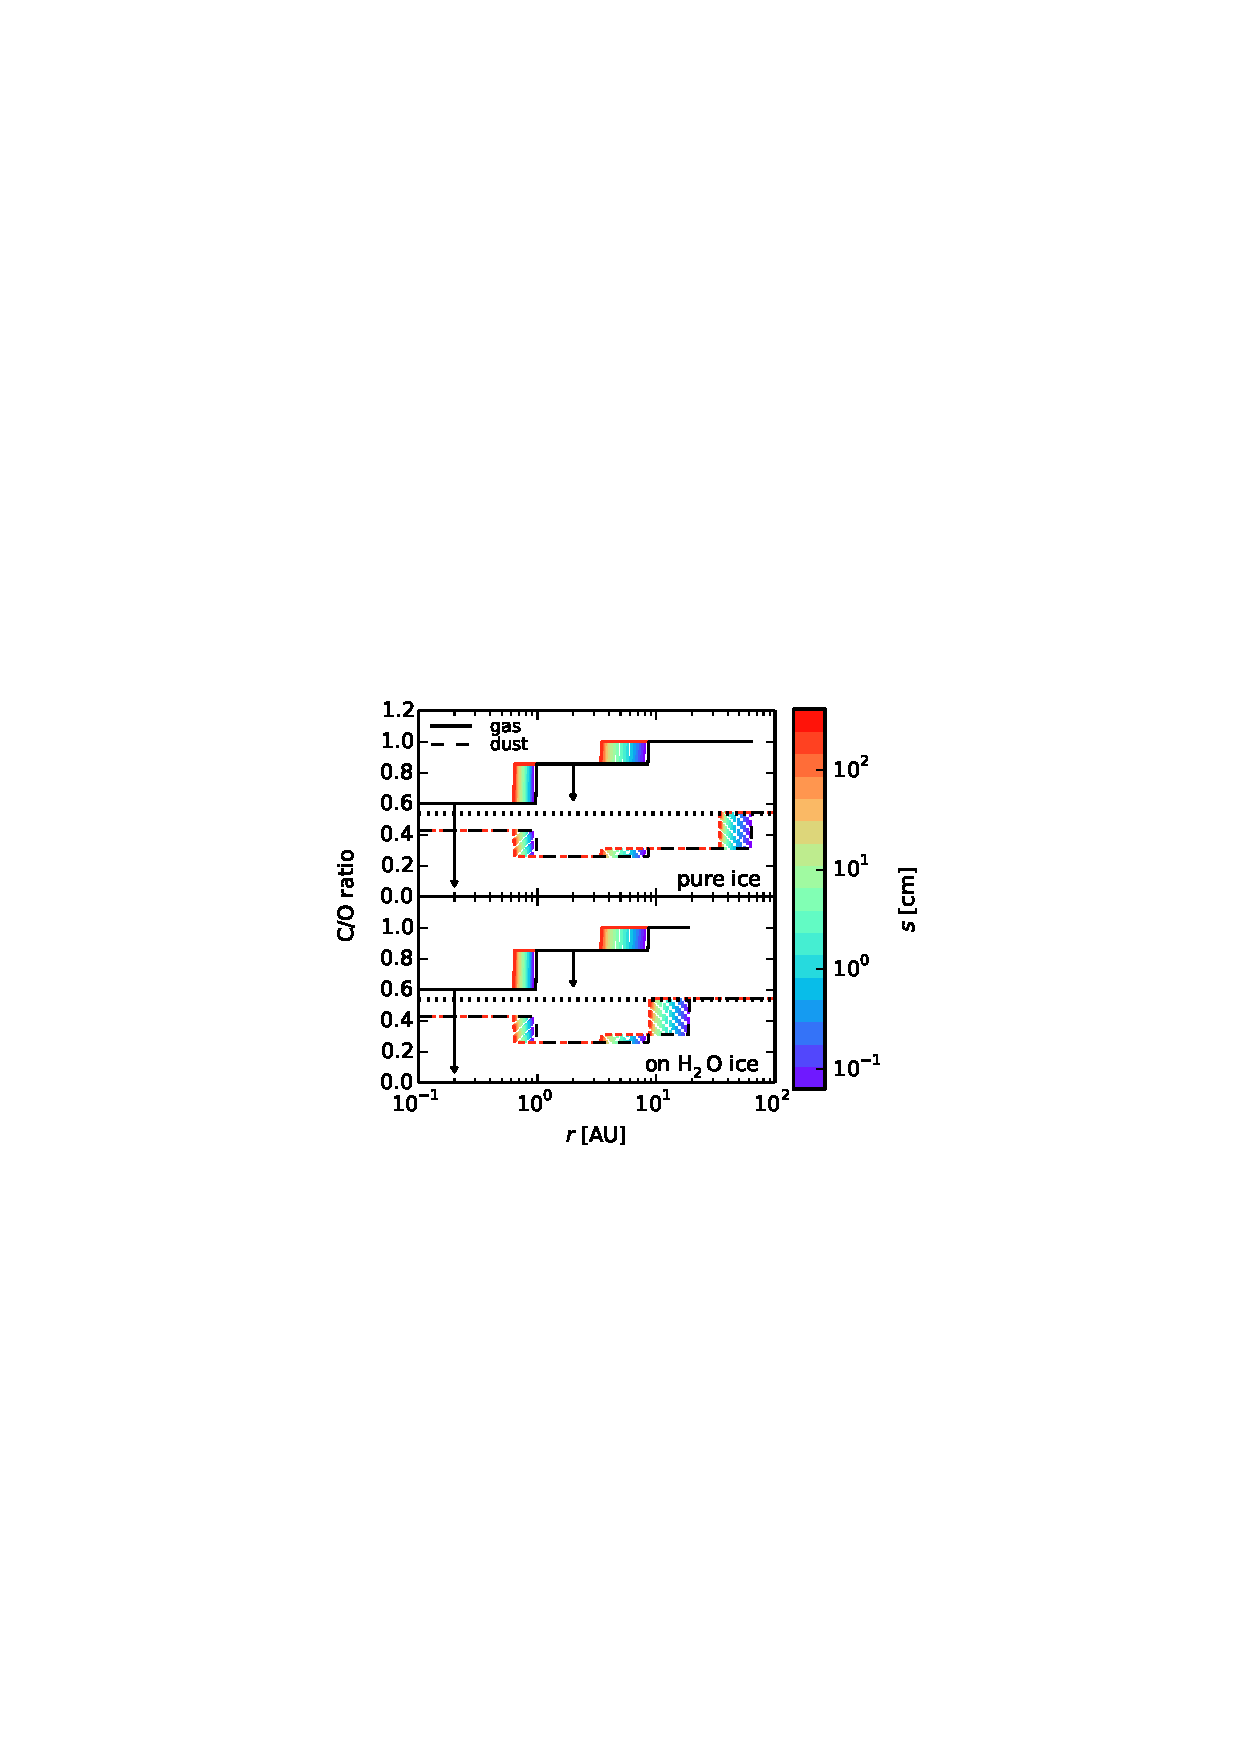
\includegraphics[width=0.5\textwidth]{../../figs/C_O_water_ice.pdf}
%\vspace{-0.5in}
\caption{C/O ratio as function of semimajor axis for CO combined with H2O (top panel) and pure CO ice (bottom panel).... Drift and gas accretion move the CO snowlines inward by x\% and y\%, respectively.} 
\label{fig:CO_ratio}
\end{figure}

\section{Nitrogen Carriers and N/O Ratios}

\emgr{Similar to the previous section, but with more details. Discuss that nitrogen is abundant in the solar system and disks and primarily found as N2. Due to the high volatility of N2, the gas phase N/O ratio in the outer disk may be even more enhanced than the C/O ratio. A fraction of the nitrogen abundance may be also carried by NH3. Discuss NH3 observed abundances and the choices that we make (no NH3, median, maximum). State that the NH3 desorption energy is only weakly dependent on whether it's pure NH3 or combined with H2O, but that is not the case for N2. Present new binding energies for N2 as pure ice and combined with water. Show Figure 4 and discuss how different nitrogen abundances and binding energies affect snowline locations and N/O ratio: N2 combined with H2O moves the N2 snowline inward by $\sim$50 AU (will calculate percentages too); the maximum reasonable abundance of NH3 changes the N/O ratio by $\sim$15\%. In the outer disk, the N/O ratio is enhanced by a factor of $\sim$4 compared to the solar value, twice as much as the C/O enhancement. Show Figure 5 and quantify the effect of drift and accretion on the NH3 snowline compared to a static disk. While NH3 does not have a significant effect on the N/O ratio in a static disk, this effect may be larger in a viscous disk, as the N gas abundance inside the NH3 snowline may be enhanced due to the differential motion of the desorbed ices and overall nebular gas (refer to Paper I). In this study, however, we neglect these effects and therefore do not include NH3 in estimating the N/O ratio (again, N/O ratio figure with drift is quite messy when including NH3 and does not add any information that is not already shown in Figures 4 and 5). Show Figure 6 and estimate the difference between N2-H2O and N2 pure ice snowlines in the case of drift, as well as the comparisons for the static disk for the N2 snowline. State that there will be an overabundance of gas-phase N/O between the CO and N2 snowlines, as there is no oxygen gas in this region.}

\begin{figure}[h!]
\centering
\includegraphics[width=0.5\textwidth]{../../figs/N_O_ratio_test.pdf}
%\vspace{-0.5in}
\caption{N/O ratio in a static disk for different NH3 abundances and N2 binding energies...} 
\label{fig:Nstatic}
\end{figure}

\begin{figure}[h!]
\centering
\includegraphics[width=0.5\textwidth]{../../figs/desorption_distance_NH3_steady.pdf}
%\vspace{-0.5in}
\caption{Desorption distance as a function of initial distance for NH3.... Drift and gas accretion move the NH3 snowline inward by x\%.} 
\label{fig:NH3}
\end{figure}

\begin{figure}[h!]
\centering
\includegraphics[width=0.5\textwidth]{../../figs/N_O_water_ice.pdf}
%\vspace{-0.5in}
\caption{N/O ratio as function of semimajor axis for N2 combined with H2O (top panel) and pure N2 ice (bottom panel).... Drift and gas accretion move the N2 snowlines inward by x\% and y\%, respectively. Overabundance of gas-phase N/O between the CO and N2 snowlines, marked by the vertical red dash-dotted lines for the largest drifting particles in our model.} 
\label{fig:NO_ratio}
\end{figure}

\section{Discussion}

\emgr{Discuss how entrapment of volatiles by H2O affects volatile abundances and C/O ratios. Re-emphasize the fact that the C/O and N/O ratios are upper estimates, and that CH4 and NH3 might matter in a viscous disk. State that we plan to address this in a future paper. More TBD.}

\section{Summary}

\emgr{Maybe we can include the summary in the discussion section?}

%\section{Volatile Abundances and Binding Energies: Effect on C/O and N/O Ratios in a Static Disk}
%
%\subsection{Nitrogen and CH4}
%
%\emgr{Discuss that nitrogen is abundant in the solar system and should be abundant in disks as well, but that its dominant form is largely unknown. Discuss that the main carrier of nitrogen is N2, but some fraction of it can be NH3 as well. Present and motivate the choices that we make for NH3 abundances. Along the same lines, discuss CH4, and the choices that we make for CH4 abundances.}
%
%\subsection{Volatile Desorption Energies}
%
%\emgr{State that desorption energies for H2O and CO2 are well constrained experimentally, and that the CO2 binding energy is only weakly dependent on whether it's pure CO2 or combined with H2O, but that is not the case for CO, N2 (and perhaps CH4 and NH3?). Briefly discuss CO-CO, N2-N2, CO-H2O and N2-H2O (and perhaps the same for CH4 and NH3 if we find literature on that) experimental results for binding energies, and motivate the choices that we make.}
%
%\subsection{Results for C/O and N/O in a Static Disk}
%
%\emgr{For each of them (C/O and N/O), show a 3-panel plot as follows: each panel has a specific CH4/NH3 abundance (top: none, middle: median abundance, bottom: maximum abundance); for a given panel, have multiple curves for C/O or N/O, depending on the choice of binding energies, so that it's clear visually how the binding energy changes the snowline location. Discuss how different abundances  and binding energies affect snowline locations and C/O or N/O ratios.}
%\section{Results}
%
%\subsection{N2, NH3 and CH4 Snowline Locations}
%
%\emgr{One multipanel 3x3 (or 3x2) rainbow plot similar to the snowline plots from Paper I, for \textit{one} choice for the binding energies (perhaps the largest ones, since we want a limit on how far in we can push the snowlines?). Rows: snowlines as a function or particle size for passive, active and (maybe) steady-state disk. Columns: N2, NH3 and CH4. Not entirely certain how necessary these plots/subsection actually are, since it is exactly the same qualitatively as in Paper I...}
%
%\subsection{C/O and N/O Ratios}
%
%\emgr{For each of them (C/O and N/O) show a 3x3 multipanel plot similar to the C/O plot from Paper I, for the same choice of binding energies as in the previous subsection. Columns: C/O or N/O in passive, active and steady-state disk. Rows: No CH4/NH3, median CH4/NH3, maximum CH4/NH3. Again, not sure if we need/want this for all disk choices, at least in the case of C/O since we already have that in Paper I. For N/O, quantify how the snowline location changes from a static disk due to drift and gas accretion.}






\if\bibinc n
\bibliography{refs}
\fi

\if\bibinc y
\begin{thebibliography}
\end{thebibliography}
\fi


\end{document}